\documentclass[journal]{IEEEtran}
\usepackage[utf8]{inputenc}
\usepackage[T1]{fontenc}
\usepackage{graphicx}
\usepackage{booktabs}
\usepackage{amsmath}
\usepackage{url}
\graphicspath{{figs/}}

\begin{document}

\title{Predicción de Riesgo de Impago Crediticio\\ utilizando Machine Learning}

\author{Oswaldo~Alejandro~Quispe~Monzón,~\IEEEmembership{Estudiante,~ML,}
        Maricielo~Patricia~Valverde~Quispe,~\IEEEmembership{Estudiante,~ML}
\thanks{Los autores son estudiantes de las carreras Ciencia de Datos y Ciencia de la Computación en la Universidad de Ingeniería y Tecnología (UTEC), Lima, Perú.}
\thanks{Proyecto de curso: Machine Learning - CS 3061. Profesor: Victor Eduardo Martínez Abaunza.}}

\maketitle

\begin{abstract}
La inclusión financiera de poblaciones sin historial crediticio exige métodos capaces de estimar el riesgo de impago a partir de datos alternativos. En este trabajo desarrollamos un pipeline completo de aprendizaje automático sobre el conjunto \textit{Home Credit Default Risk} (307{,}511 solicitudes distribuidas en siete tablas relacionales): auditoría y limpieza de datos, ingeniería de características por agregación (253 variables finales) y comparación de ocho configuraciones de modelos, desde regresión logística hasta \textit{gradient boosting} y un perceptrón multicapa. El mejor modelo, un LightGBM ajustado mediante optimización bayesiana, alcanza un AUC de 0.7882 sobre un conjunto de validación intacto. El análisis se complementa con interpretabilidad SHAP y una auditoría de equidad algorítmica por género y edad, que ilustra empíricamente el teorema de imposibilidad de la equidad y evalúa una mitigación de igualdad de oportunidad. Los resultados muestran que la señal predictiva proviene de combinar muchos predictores individualmente débiles.
\end{abstract}

\begin{IEEEkeywords}
Machine Learning, credit scoring, riesgo crediticio, default, Home Credit, LightGBM, SHAP, equidad algorítmica.
\end{IEEEkeywords}

\section{Introducción}

\IEEEPARstart{E}{l} acceso al crédito es un motor fundamental para el desarrollo económico individual; sin embargo, las instituciones financieras tradicionales suelen rechazar a solicitantes sin un historial crediticio suficiente. Esto genera una barrera significativa para la población no bancarizada (\textit{unbanked}). Para enfrentar este problema, entidades como Home Credit utilizan datos alternativos, como información de telecomunicaciones y comportamiento transaccional, para evaluar la capacidad de pago. El reto consiste en extraer patrones predictivos precisos de datos heterogéneos y desbalanceados para tomar decisiones de préstamo seguras.

Los objetivos de este proyecto son: (i) realizar un análisis exploratorio de datos (EDA) estructurado sobre el ecosistema relacional completo para identificar las variables más asociadas a la capacidad de pago; (ii) desarrollar y comparar modelos de clasificación supervisada ---regresión logística, árboles de decisión, Random Forest, XGBoost, LightGBM y una red neuronal multicapa--- para predecir la probabilidad de impago; (iii) evaluar el rendimiento con métricas adecuadas para clases desbalanceadas, principalmente el área bajo la curva ROC (AUC); y (iv) auditar la interpretabilidad y la equidad algorítmica del modelo final, dimensión crítica para el despliegue responsable de sistemas de \textit{credit scoring}.

Se utilizó el dataset \textit{Home Credit Default Risk} de la plataforma Kaggle. Este conjunto proporciona información histórica de solicitudes de préstamo organizada en una tabla principal (\texttt{application\_train/test}, con la variable objetivo \texttt{TARGET}: 1 = impago) y seis tablas relacionales secundarias que detallan el historial del cliente en el buró de crédito y dentro de la propia institución. La unidad de predicción es la solicitud (\texttt{SK\_ID\_CURR}) y el problema es de clasificación binaria con desbalance moderado: solo el 8.07\% de las 307{,}511 solicitudes de entrenamiento corresponde a impagos (razón 11.4:1).

\section{Revisión Bibliográfica}

La predicción de riesgo crediticio o \textit{credit scoring} ha evolucionado significativamente con la adopción del \textit{Machine Learning}, y la literatura orienta directamente las decisiones metodológicas de este proyecto.

\subsection{Modelos y benchmarks para credit scoring}

Lessmann \textit{et al.} \cite{lessmann2015} realizaron una evaluación comparativa exhaustiva de algoritmos de clasificación para \textit{credit scoring}, demostrando que los ensambles basados en árboles superan consistentemente a los modelos estadísticos tradicionales. Este hallazgo justifica centrar la comparación en ensambles, con la regresión logística como línea base. Khandani \textit{et al.} \cite{khandani2010} demostraron que modelos entrenados sobre datos transaccionales de consumidores pueden reducir sustancialmente las tasas de morosidad, un enfoque directamente aplicable al tipo de información conductual que incorpora Home Credit. Brown y Mues \cite{brown2012} concluyeron experimentalmente que Random Forest y \textit{gradient boosting} son particularmente robustos ante el desbalance de clases, lo que guía tanto la selección de modelos como la elección del AUC como métrica principal. Dastile \textit{et al.} \cite{dastile2020} destacaron en su revisión sistemática la explicabilidad como criterio fundamental de adopción en el sector financiero, motivando la inclusión de modelos interpretables junto a los complejos. Breiman \cite{breiman2001} formalizó Random Forest y el mecanismo por el cual el \textit{bagging} de árboles descorrelacionados reduce la varianza sin aumentar el sesgo, fundamento teórico del contraste sesgo--varianza que estructura nuestra comparativa experimental.

\subsection{Gradient boosting y optimización de hiperparámetros}

Chen y Guestrin \cite{chen2016} introdujeron XGBoost, el sistema de \textit{boosting} escalable con regularización explícita que popularizó esta familia en competencias de datos tabulares. Ke \textit{et al.} \cite{ke2017} propusieron LightGBM, que mediante histogramas, crecimiento \textit{leaf-wise} y manejo nativo de variables categóricas logra mayor eficiencia con igual o mejor precisión; ambas propiedades resultaron decisivas para entrenar sobre 253 características y 307 mil filas con hardware limitado. Xia \textit{et al.} \cite{xia2017} propusieron la optimización bayesiana de hiperparámetros para \textit{boosting} en \textit{credit scoring}, logrando mejoras significativas en AUC; seguimos esa línea utilizando Optuna \cite{akiba2019}, un framework moderno de optimización secuencial basada en el estimador TPE. He y García \cite{he2009} sistematizaron el aprendizaje con clases desbalanceadas; de su análisis se desprende que las métricas basadas en ranking como el AUC son robustas al desbalance, lo que fundamenta nuestra decisión de no re-ponderar durante el entrenamiento y trasladar el tratamiento del desbalance al umbral de decisión. Gunnarsson \textit{et al.} \cite{gunnarsson2021} evaluaron redes profundas para \textit{credit scoring} concluyendo que no superan al \textit{boosting} en datos tabulares, conclusión que nuestro experimento con un perceptrón multicapa replica.

\subsection{Interpretabilidad y equidad algorítmica}

Lundberg y Lee \cite{lundberg2017} unificaron los métodos de atribución aditiva en el marco SHAP, basado en valores de Shapley, que empleamos para explicar el modelo final. En cuanto a equidad, Hardt \textit{et al.} \cite{hardt2016} propusieron el criterio de igualdad de oportunidad (igual tasa de verdaderos positivos entre grupos) y su implementación mediante umbrales específicos por grupo, que es exactamente la mitigación que evaluamos. Kleinberg \textit{et al.} \cite{kleinberg2017} demostraron formalmente que, cuando las tasas base difieren entre grupos, la calibración y el balance de errores no pueden satisfacerse simultáneamente (teorema de imposibilidad), resultado que observamos empíricamente. Kozodoi \textit{et al.} \cite{kozodoi2022} trasladaron estos criterios al dominio específico del \textit{credit scoring}, cuantificando el costo en beneficio de imponer equidad y concluyendo que criterios distintos implican trade-offs distintos; su marco informa nuestra discusión del costo en precisión de la mitigación.

\section{Metodología}

\subsection{Dataset y auditoría inicial}

El dataset se compone de siete tablas de datos (más un diccionario de columnas), resumidas en la Tabla~\ref{tab:dataset}. Las tablas secundarias guardan relación 1:N con la solicitud: un cliente puede tener hasta 116 créditos previos en el buró y hasta 96 meses de historial mensual. La auditoría inicial no encontró filas duplicadas; los ocho archivos se convirtieron a formato Parquet con reducción de tipos numéricos (\textit{downcasting}), disminuyendo la memoria en $\sim$50\% y permitiendo trabajar todo el proyecto con 16 GB de RAM.

\begin{table}[!t]
\caption{Inventario del dataset Home Credit Default Risk}
\label{tab:dataset}
\centering
\small
\begin{tabular}{lrr}
\toprule
Tabla & Filas & Columnas \\
\midrule
application\_train & 307{,}511 & 122 \\
application\_test & 48{,}744 & 121 \\
bureau & 1{,}716{,}428 & 17 \\
bureau\_balance & 27{,}299{,}925 & 3 \\
previous\_application & 1{,}670{,}214 & 37 \\
POS\_CASH\_balance & 10{,}001{,}358 & 8 \\
credit\_card\_balance & 3{,}840{,}312 & 23 \\
installments\_payments & 13{,}605{,}401 & 8 \\
\bottomrule
\end{tabular}
\end{table}

\subsection{Limpieza y análisis exploratorio}

La limpieza abordó tres tipos de anomalías. Primero, el valor centinela $365243$ en las columnas \texttt{DAYS\_*}: nuestra primera lectura fue tratarlo como ruido de captura, pero al cruzar las 55{,}374 filas afectadas en \texttt{DAYS\_EMPLOYED} (18.0\%) con el tipo de ocupación resultó lo contrario ---son casi íntegramente pensionistas, un grupo que impaga menos que el resto (5.40\% vs.\ 8.66\%). La anomalía no era un error: era información, y la conservamos como indicador binario antes de anular el valor. Segundo, las categorías centinela \texttt{XNA}/\texttt{XAP} se trataron como nulos. Tercero, se eliminaron 39 columnas redundantes de \texttt{application} (los bloques inmobiliarios \texttt{\_MODE} y \texttt{\_MEDI}, con correlación interna media de 0.983 respecto de \texttt{\_AVG}; nueve indicadores de documentos con activación menor a 0.1\%; y una columna constante), además de variables derivadas con correlación $\approx$ $-1.00$ con su original.

El EDA se organizó por tablas y familias de variables. Como criterio de poder predictivo consideramos primero la información mutua y terminamos descartándola: en columnas imputadas con centinela, lo que se vuelve informativo es la \emph{nulidad} y no el valor, de modo que el ranking premia artificialmente a las columnas con más nulos. Adoptamos en su lugar el AUC univariado con corrección de dirección, $\max(\text{AUC}, 1-\text{AUC})$. Los hallazgos centrales fueron: (1) los puntajes externos \texttt{EXT\_SOURCE\_1/2/3} son los predictores individuales más fuertes (AUC 0.66--0.68) y están poco correlacionados entre sí (0.11--0.21), aportando tres señales casi independientes (Fig.~\ref{fig:ext}); (2) el impago decrece monótonamente con la edad, de 12.3\% en menores de 25 años a 4.9\% en 60--70 (Fig.~\ref{fig:age}); (3) en todas las tablas de historial domina la \emph{recencia y longitud} del historial sobre los montos y la morosidad puntual; (4) la utilización de la tarjeta de crédito (saldo/límite) es el segundo mejor predictor del proyecto; y (5) los eventos de mora (DPD) agregados son débiles en todas las tablas mensuales (AUC $\sim$0.50--0.55), y no porque la mora no importe: los eventos son raros y el promedio los diluye.

\begin{figure}[!t]
\centering
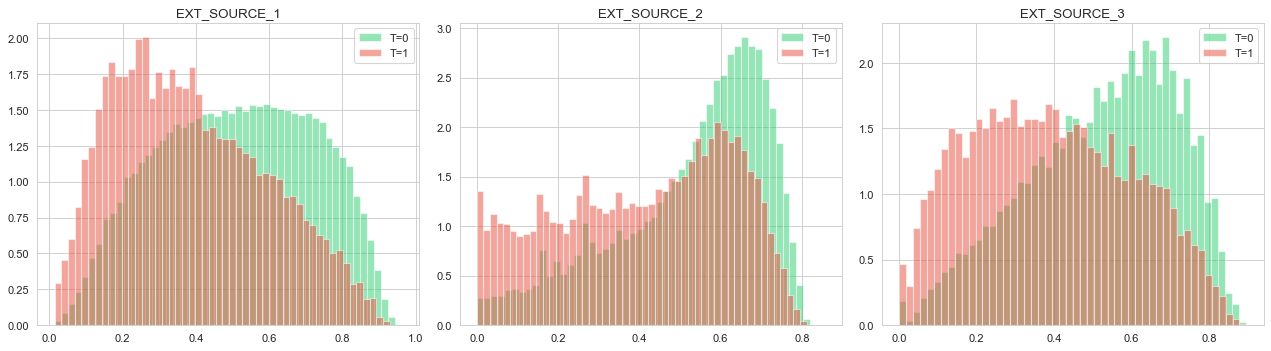
\includegraphics[width=\columnwidth]{univar_ext_sources.png}
\caption{Distribución de los puntajes externos \texttt{EXT\_SOURCE\_1/2/3} por clase. Son los predictores individuales más fuertes y mutuamente poco correlacionados.}
\label{fig:ext}
\end{figure}

\begin{figure}[!t]
\centering
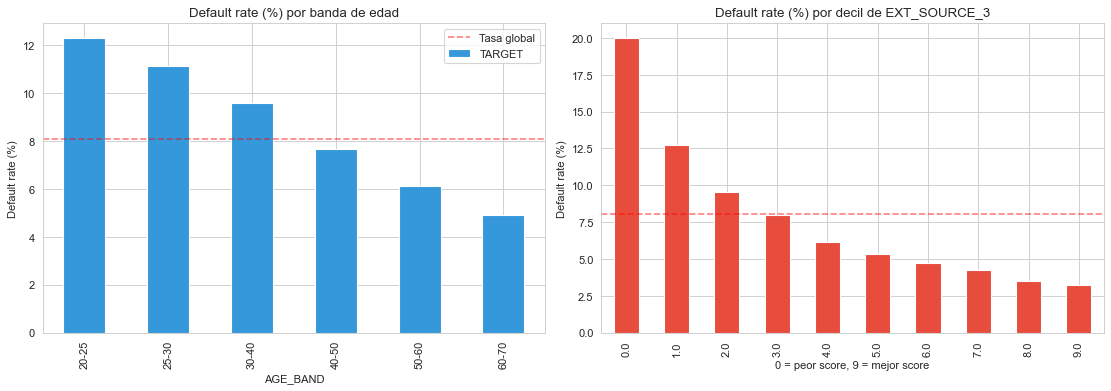
\includegraphics[width=\columnwidth]{bivar_age_ext3.png}
\caption{Tasa de impago por banda de edad (monótona decreciente) y por decil de \texttt{EXT\_SOURCE\_3} (del 20.0\% en el peor decil al 3.2\% en el mejor).}
\label{fig:age}
\end{figure}

\subsection{Ingeniería de características por agregación}

Dado que las tablas secundarias tienen granularidad crédito--mes, se construyeron características a nivel de cliente mediante agregaciones estadísticas (media, mínimo, máximo, suma, conteos y proporciones), incluyendo variables de dominio como la utilización de tarjeta (\texttt{AMT\_BALANCE}/\texttt{AMT\_CREDIT\_LIMIT\_ACTUAL}), la puntualidad de pago de cuotas (días de atraso y razón pagado/exigido, tratando cuotas sin pago como impago total) y las razones aprobado/solicitado de créditos previos. \texttt{bureau\_balance} requirió agregación en dos niveles (crédito $\rightarrow$ cliente). En total se generaron 24 características del buró, 25 de su historial mensual, 37 de solicitudes previas, 25 de POS, 31 de tarjeta y 23 de cuotas. Como la cobertura de las tablas varía (del 94.8\% de \texttt{installments} al 28.3\% de \texttt{credit\_card}), decidimos no tratar la ausencia de historial como un hueco que imputar sino como información en sí misma (\textit{thin file}): banderas \texttt{HAS\_*} creadas antes del \textit{join} capturan los nulos estructurales de las columnas agregadas sin necesidad de indicadores por columna. El \textit{merge} maestro se realizó con \textit{left joins} 1:1 validados, resultando en matrices de 307{,}511 $\times$ 253 (train) y 48{,}744 $\times$ 252 (test) con paridad exacta de columnas salvo \texttt{TARGET}.

\subsection{Protocolo experimental}

Nos impusimos una regla desde el inicio: apartar un conjunto de validación estratificado del 20\% (61{,}503 solicitudes) y no tocarlo hasta la evaluación final. Toda decisión que requería mirar datos se resolvió dentro del 80\% restante: los hiperparámetros, con validación cruzada estratificada de 5 particiones; el umbral de decisión, con predicciones \textit{out-of-fold} (OOF) del mismo conjunto. La métrica principal es el AUC-ROC, robusta al desbalance y independiente del umbral \cite{he2009,brown2012}; la exactitud se descartó por trivial ($\approx$92\% prediciendo siempre la clase mayoritaria).

Se emplearon dos preprocesamientos según la familia de modelo. Para los modelos lineales y la red neuronal: imputación por mediana y estandarización en numéricas; \textit{one-hot} para categóricas de baja cardinalidad; y \textit{target encoding} con ajuste cruzado (para evitar fuga de información) en las dos de alta cardinalidad, totalizando 302 columnas. Para los modelos de árboles: codificación ordinal con categoría explícita para nulos y numéricas crudas sin imputar; LightGBM utilizó adicionalmente sus particiones categóricas nativas.

\subsection{Modelos implementados y justificación}

La selección de modelos sigue una progresión pedagógica del trade-off sesgo--varianza y las recomendaciones de la literatura \cite{lessmann2015,brown2012}: (a) \textbf{regresión logística} con regularización L2 como línea base interpretable y auditable \cite{dastile2020}; (b) \textbf{árbol de decisión} en dos versiones ---podado a profundidad 5 y sin restricciones--- para exhibir el sobreajuste de un estimador de alta varianza; (c) \textbf{Random Forest} \cite{breiman2001} como reducción de varianza vía \textit{bagging}; (d) \textbf{XGBoost} \cite{chen2016} y (e) \textbf{LightGBM} \cite{ke2017} como reducción de sesgo vía \textit{boosting}. El primer informe contemplaba XGBoost como modelo principal; lo mantuvimos como punto de comparación con configuración equivalente, pero adoptamos LightGBM como candidato final por su manejo nativo de categóricas y su menor costo computacional a esta escala. (f) Finalmente, un \textbf{perceptrón multicapa} (MLP, capas ocultas 64--32, ReLU, Adam, regularización L2 $\alpha=10^{-2}$ y parada temprana) cubre la familia de redes neuronales y permite contrastar la evidencia de que el aprendizaje profundo no supera al \textit{boosting} en tabular \cite{gunnarsson2021}.

Nuestra intuición inicial para el desbalance era la receta estándar: re-ponderar la clase minoritaria (\texttt{scale\_pos\_weight} = 11.4). El experimento la contradijo: el \textit{boosting} re-ponderado colapsa (parada temprana en 1--3 iteraciones) y pierde 65 milésimas de AUC frente a la versión sin pesos. La explicación es que el AUC ordena en lugar de clasificar y es invariante al umbral: el desbalance no se combate en el entrenamiento sino en la decisión, así que trasladamos su tratamiento íntegramente al umbral.

Los hiperparámetros de LightGBM se ajustaron con Optuna \cite{akiba2019,xia2017}: 114 \textit{trials} en 180 minutos, cada uno evaluado con validación cruzada completa de 5 particiones sobre ocho hiperparámetros (hojas, muestras mínimas por hoja, submuestreo de filas y columnas, regularización L1/L2 y ganancia mínima de partición). La configuración ganadora es fuertemente regularizada (\texttt{num\_leaves}=16, \texttt{min\_child\_samples}=104, $\lambda_1$=9.01, $\lambda_2$=9.94, \texttt{feature\_fraction}=0.56), consistente con un problema cuya señal proviene de muchos predictores débiles.

\subsection{Auditoría de interpretabilidad y equidad}

El modelo final se explicó con SHAP (TreeExplainer) sobre una muestra de validación \cite{lundberg2017}. La equidad se auditó por género y edad con métricas por grupo: calibración (probabilidad media predicha vs.\ tasa real), AUC, tasa de señalamiento, TPR (igualdad de oportunidad \cite{hardt2016}), FPR y precisión. Se evaluaron además dos intervenciones: umbrales por grupo para igualar TPR \cite{hardt2016} y el retiro del atributo protegido (\textit{fairness through unawareness}).

\section{Resultados}

\subsection{Comparativa de modelos}

La Tabla~\ref{tab:models} resume el desempeño sobre el conjunto de validación intacto. El árbol sin podar ilustra la varianza extrema (AUC 0.9943 en entrenamiento y 0.5387 en validación, con profundidad 103 y 22{,}634 hojas); su versión podada generaliza pero con sesgo alto. Random Forest elimina la varianza del árbol (0.7675) y el \textit{boosting} reduce además el sesgo: XGBoost alcanza 0.7858 y LightGBM 0.7849 sin ajuste. El ajuste bayesiano eleva LightGBM a \textbf{0.7882} (validación cruzada: 0.7861 vs.\ 0.7835 sin ajustar), el mejor resultado del proyecto, con intervalo de confianza bootstrap del 95\% de $[0.781, 0.794]$ sobre validación. Cabe precisar que XGBoost y el MLP se evaluaron con configuraciones estándar sin búsqueda exhaustiva de hiperparámetros, por lo que la comparación con el LightGBM ajustado favorece a este último; la comparación justa es contra LightGBM sin ajustar (0.7858 vs.\ 0.7849, diferencia dentro del ruido muestral). Dos resultados nos parecen más informativos que el propio ganador. El primero: la regresión logística queda a solo 13 milésimas del mejor modelo (0.7749 vs.\ 0.7882); gran parte de la señal es, en la práctica, lineal y monótona, dominada por los \texttt{EXT\_SOURCE}. El segundo contradijo nuestra expectativa sobre las redes neuronales: el MLP (0.7701) no alcanza siquiera a la línea base logística pese a contar con muchos más parámetros, replicando sobre nuestros datos la conclusión de \cite{gunnarsson2021} para tabular de crédito.

\begin{table}[!t]
\caption{Comparativa de modelos sobre validación intacta (20\%)}
\label{tab:models}
\centering
\small
\begin{tabular}{lccc}
\toprule
Modelo & AUC train & AUC val & Gap \\
\midrule
Regresión logística (L2) & 0.7763 & 0.7749 & +0.0014 \\
Árbol de decisión (prof.\ 5) & 0.7166 & 0.7131 & +0.0035 \\
Árbol sin podar & 0.9943 & 0.5387 & +0.4556 \\
Random Forest & 0.9836 & 0.7675 & +0.2161 \\
MLP (64--32) & 0.8024 & 0.7701 & +0.0323 \\
XGBoost (sin ajustar) & 0.8655 & 0.7858 & +0.0798 \\
LightGBM (sin ajustar) & 0.8840 & 0.7849 & +0.0991 \\
\textbf{LightGBM ajustado} & 0.8514 & \textbf{0.7882} & +0.0632 \\
\bottomrule
\end{tabular}
\end{table}

\subsection{Umbral de decisión como palanca de política}

Las probabilidades del modelo se concentran alrededor de la tasa base (8\%), por lo que el umbral estándar de 0.5 es inservible. El umbral que maximiza F1, estimado honestamente con predicciones OOF de entrenamiento, es 0.172. Aplicado a validación, el modelo señala 7{,}288 solicitudes (11.8\%) con precisión 0.288 ---un \textit{lift} de 3.6$\times$ sobre la tasa base--- y recall 0.424. La curva precisión--recall (Fig.~\ref{fig:prroc}) muestra el trade-off disponible: capturar el 50\% de los impagos exige aceptar precisión 0.260; el 70\%, precisión 0.188; y el 80\%, precisión 0.157. En un contexto donde el costo de un impago no detectado supera con creces el de una revisión adicional, el umbral operativo debería favorecer el recall: es una decisión de política de negocio, no un parámetro técnico.

\begin{figure}[!t]
\centering
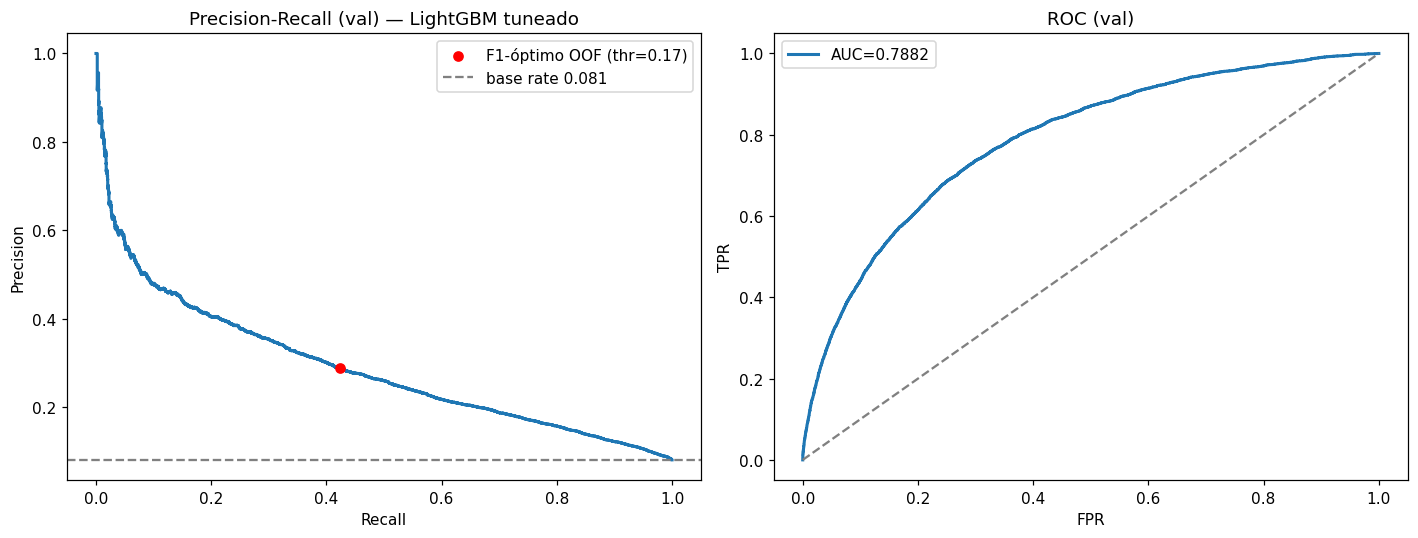
\includegraphics[width=\columnwidth]{pr_roc_lgbm_tuned.png}
\caption{Curvas precisión--recall y ROC del LightGBM ajustado sobre validación. El punto marca el umbral F1-óptimo (0.172) estimado con OOF de entrenamiento.}
\label{fig:prroc}
\end{figure}

\subsection{Interpretabilidad}

El análisis SHAP (Fig.~\ref{fig:shap}) confirma la jerarquía del EDA: \texttt{EXT\_SOURCE\_2} (0.298), \texttt{EXT\_SOURCE\_3} (0.255) y \texttt{EXT\_SOURCE\_1} (0.144) dominan, seguidas de los montos del crédito (\texttt{AMT\_GOODS\_PRICE}, \texttt{AMT\_ANNUITY}, \texttt{AMT\_CREDIT}) y de características de comportamiento construidas en la agregación, como la proporción de cuotas pagadas tarde (\texttt{INST\_IS\_LATE\_MEAN}). La dependencia de \texttt{EXT\_SOURCE\_3} es monótona decreciente y trata su ausencia como riesgo elevado (Fig.~\ref{fig:dep}). El modelo valida además dos hallazgos de negocio. Uno esperable: la utilización de tarjeta y los avances en efectivo por cajero como señales de estrés financiero. Otro contraintuitivo, quizá el hallazgo menos obvio del proyecto: los clientes a quienes se aprobó \emph{más} de lo que solicitaron impagan más ---el \textit{upselling}, visto desde el riesgo, es un anti-patrón. De modo crítico para la siguiente subsección, \texttt{CODE\_GENDER} ocupa el puesto \#6 de 251 características (|SHAP| medio 0.113): el modelo se apoya directamente en un atributo protegido.

\begin{figure}[!t]
\centering
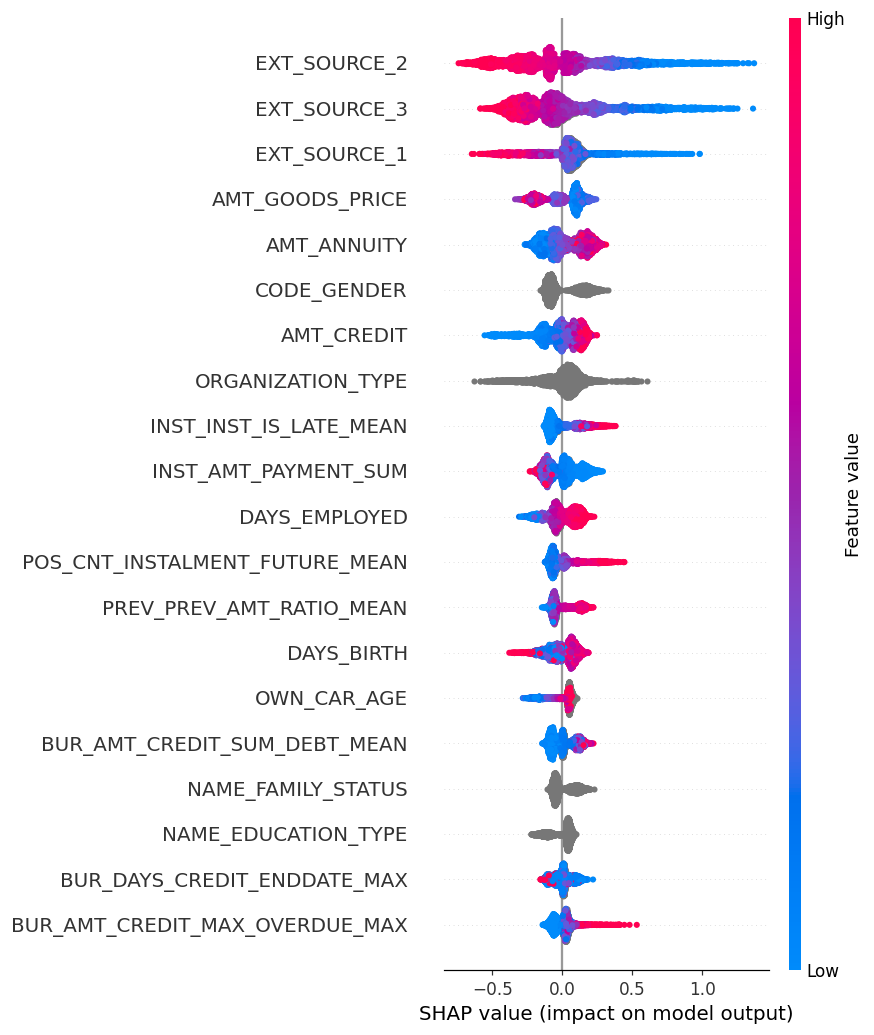
\includegraphics[width=\columnwidth]{shap_summary.png}
\caption{Resumen SHAP del modelo final (20 características principales).}
\label{fig:shap}
\end{figure}

\begin{figure}[!t]
\centering
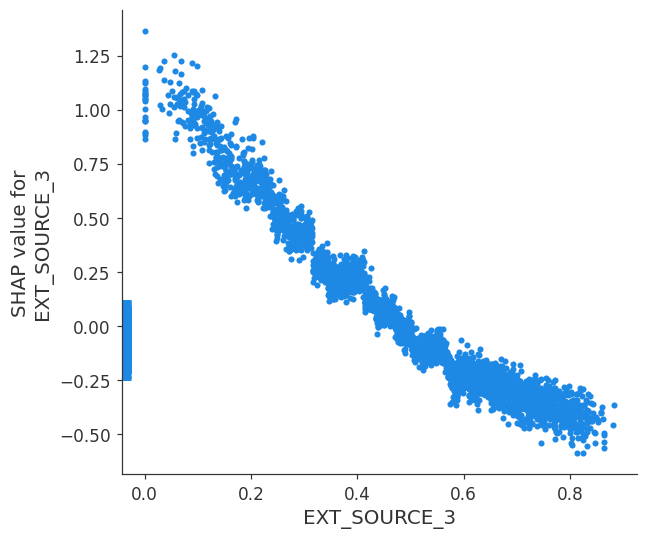
\includegraphics[width=\columnwidth]{shap_dep_ext3.png}
\caption{Dependencia SHAP de \texttt{EXT\_SOURCE\_3}: efecto monótono decreciente; los valores ausentes se asocian a riesgo elevado.}
\label{fig:dep}
\end{figure}

\subsection{Equidad algorítmica}

La Tabla~\ref{tab:fairness} presenta la auditoría por género al umbral 0.172. El modelo está bien calibrado en ambos grupos (probabilidad media predicha $\approx$ tasa real de impago) y su AUC es prácticamente igual (F: 0.7830, M: 0.7854). Sin embargo, como las tasas base difieren (F: 7.0\%, M: 10.1\%), a umbral fijo divergen el TPR (0.370 vs.\ 0.496) y el FPR (0.072 vs.\ 0.131): las mujeres impagadoras son detectadas con menor frecuencia y los hombres cumplidores son señalados en falso con mayor frecuencia. Esto no es un defecto de implementación sino la manifestación empírica del teorema de imposibilidad \cite{kleinberg2017}: con tasas base distintas, calibración e igualdad simultánea de TPR y FPR son matemáticamente incompatibles.

\begin{table}[!t]
\caption{Auditoría de equidad por género (umbral 0.172, validación)}
\label{tab:fairness}
\centering
\small
\begin{tabular}{lcc}
\toprule
Métrica & Mujeres (F) & Hombres (M) \\
\midrule
Tasa real de impago & 0.070 & 0.101 \\
Prob.\ media predicha & 0.070 & 0.100 \\
AUC & 0.7830 & 0.7854 \\
Tasa de señalamiento & 0.093 & 0.168 \\
Recall (TPR) & 0.370 & 0.496 \\
FPR & 0.072 & 0.131 \\
Precisión & 0.277 & 0.299 \\
\bottomrule
\end{tabular}
\end{table}

Por edad, el modelo también está calibrado, pero el AUC cae en los extremos ($<$25: 0.747; 60+: 0.745), consistente con historiales delgados y mayor homogeneidad, y la tasa de señalamiento decrece $\approx$6$\times$ entre el grupo más joven y el mayor (0.234 $\rightarrow$ 0.038), reflejo del gradiente real de riesgo por edad.

Se evaluaron dos mitigaciones. Primero, igualdad de oportunidad \cite{hardt2016}: umbrales por grupo calibrados en OOF de entrenamiento (F: 0.139, M: 0.184) para igualar el TPR en $\sim$0.45 producen un desempeño global de precisión 0.270 y recall 0.458; igualar la oportunidad tiene un costo directo en precisión, cuantificando el trade-off entre eficiencia y equidad \cite{kozodoi2022}. Segundo, \textit{unawareness}: la solución aparentemente obvia ---retirar \texttt{CODE\_GENDER} del modelo--- resultó ser la menos efectiva. Cuesta solo 0.0018 de AUC (0.7882 $\rightarrow$ 0.7864), pero el gap de probabilidad predicha entre géneros apenas se reduce de 0.0300 a 0.0204 (gap real: 0.0318): las variables correlacionadas reconstruyen $\sim$68\% de la señal. Quitar el género del modelo no lo quita de los datos; es necesario para evitar el trato dispar directo, pero insuficiente como garantía de equidad.

\subsection{Validación externa en Kaggle}

El modelo final, reentrenado sobre el 80\% de entrenamiento con los hiperparámetros óptimos y 983 iteraciones, generó predicciones para las 48{,}744 solicitudes de test (probabilidad media 0.0716, coherente con la tasa base y con el hecho, detectado en el EDA, de que los clientes de test tienen historial más rico: 98.1\% con solicitudes previas vs.\ 94.7\% en entrenamiento). Estas predicciones se evaluaron externamente en la plataforma Kaggle, cuyo conjunto de test posee etiquetas que nunca estuvieron disponibles durante el desarrollo, obteniendo un AUC de \textbf{0.78309} en el \textit{leaderboard} público y \textbf{0.77958} en el privado. La distancia entre la estimación interna (0.7882) y el resultado externo es de nueve milésimas: la firma de un protocolo sin fugas, en el que nada del conjunto de validación se filtró al desarrollo. Como referencia, la solución ganadora de la competencia alcanzó 0.80570 en el \textit{leaderboard} privado utilizando ensambles masivos de decenas de modelos.

\section{Conclusiones}

Construir un pipeline completo de \textit{credit scoring} sobre un ecosistema relacional de más de 58 millones de registros ---doce cuadernos, un modelo final validado externamente--- nos deja cinco conclusiones. Primera: en datos tabulares heterogéneos, el \textit{gradient boosting} regularizado sigue siendo el estado de la práctica; LightGBM ajustado (AUC 0.7882) superó a todas las alternativas, incluido un MLP, en línea con la literatura \cite{lessmann2015,gunnarsson2021}. Segunda: la comparativa materializa el trade-off sesgo--varianza: el árbol sin podar memoriza (gap +0.456), el \textit{bagging} elimina varianza y el \textit{boosting} reduce sesgo; y la competitividad de la regresión logística (0.7749) revela que la mayor parte de la señal es monótona y aproximadamente lineal. Tercera: la ingeniería de características por agregación importa tanto como el modelo: las señales de comportamiento construidas (utilización de tarjeta, recencia del historial, puntualidad de cuotas, razón aprobado/solicitado) aparecen entre las variables más influyentes del SHAP, y la ausencia de historial es en sí misma información (\textit{thin file}). Cuarta: con 8\% de positivos, el desbalance se gestiona mejor en la decisión que en el entrenamiento: re-ponderar clases degradó el AUC del \textit{boosting}, mientras que la elección del umbral con OOF preservó la validez del conjunto de validación y expuso el trade-off precisión--recall como decisión de política. Quinta: un modelo calibrado y con igual AUC entre grupos puede aun así producir tasas de error desiguales cuando las tasas base difieren; la equidad no se resuelve eliminando el atributo protegido (los proxies reconstruyen dos tercios del gap) sino que exige elegir explícitamente qué criterio igualar y asumir su costo.

\section{Trabajo Futuro}

Tres extensiones mejorarían el modelo. En características: explotar señal aún no aprovechada, como los motivos de rechazo de solicitudes previas (\texttt{CODE\_REJECT\_REASON}), tendencias temporales dentro del historial mensual (pendientes de utilización o de mora en lugar de promedios, que diluyen los eventos raros) y razones de dominio adicionales (cuota/ingreso, crédito/ingreso). En modelos: ensamblar LightGBM con XGBoost y la regresión logística vía \textit{stacking}; explorar arquitecturas profundas específicas para tabular (TabNet, FT-Transformer) que aprenden agregaciones directamente de las tablas crudas; y calibrar las probabilidades (Platt/isotónica) si se requieren estimaciones de riesgo absolutas. En datos y despliegue: validar la estabilidad temporal con particiones por fecha (el EDA detectó corrimiento de distribución entre train y test), incorporar los costos monetarios reales de FN/FP para optimizar el umbral por utilidad esperada en lugar de F1, y formalizar la auditoría de equidad como restricción del entrenamiento (por ejemplo, con regularizadores de equidad \cite{kozodoi2022}) en lugar de post-procesamiento.

\section*{Código implementado}

El código completo del proyecto (12 notebooks: auditoría, limpieza, EDA por tabla, agregaciones, \textit{merge} maestro, modelado, interpretabilidad y equidad) está disponible en: \url{https://github.com/oswaldoaqm/ML-Proyecto-CreditRisk}.

\begin{thebibliography}{15}

\bibitem{lessmann2015}
S. Lessmann, B. Baesens, H. Seow, y L. C. Thomas, ``Benchmarking state-of-the-art classification algorithms for credit scoring: An update of research,'' \textit{European Journal of Operational Research}, vol. 247, no. 1, pp. 124--136, 2015.

\bibitem{khandani2010}
A. E. Khandani, A. J. Kim, y A. W. Lo, ``Consumer credit-risk models via machine-learning algorithms,'' \textit{Journal of Banking \& Finance}, vol. 34, no. 11, pp. 2767--2787, 2010.

\bibitem{brown2012}
I. Brown y C. Mues, ``An experimental comparison of classification algorithms for imbalanced credit scoring data sets,'' \textit{Expert Systems with Applications}, vol. 39, no. 3, pp. 3446--3453, 2012.

\bibitem{dastile2020}
X. Dastile, T. Celik, y M. Potsane, ``Statistical and machine learning models in credit scoring: A systematic literature survey,'' \textit{Applied Soft Computing}, vol. 91, p. 106263, 2020.

\bibitem{xia2017}
Y. Xia, C. Liu, Y. Li, y N. Liu, ``A boosted decision tree approach using Bayesian hyper-parameter optimization for credit scoring,'' \textit{Expert Systems with Applications}, vol. 78, pp. 225--241, 2017.

\bibitem{breiman2001}
L. Breiman, ``Random forests,'' \textit{Machine Learning}, vol. 45, no. 1, pp. 5--32, 2001.

\bibitem{chen2016}
T. Chen y C. Guestrin, ``XGBoost: A scalable tree boosting system,'' en \textit{Proc. 22nd ACM SIGKDD Int. Conf. on Knowledge Discovery and Data Mining}, 2016, pp. 785--794.

\bibitem{ke2017}
G. Ke \textit{et al.}, ``LightGBM: A highly efficient gradient boosting decision tree,'' en \textit{Advances in Neural Information Processing Systems 30}, 2017, pp. 3146--3154.

\bibitem{akiba2019}
T. Akiba, S. Sano, T. Yanase, T. Ohta, y M. Koyama, ``Optuna: A next-generation hyperparameter optimization framework,'' en \textit{Proc. 25th ACM SIGKDD Int. Conf. on Knowledge Discovery and Data Mining}, 2019, pp. 2623--2631.

\bibitem{he2009}
H. He y E. A. Garcia, ``Learning from imbalanced data,'' \textit{IEEE Transactions on Knowledge and Data Engineering}, vol. 21, no. 9, pp. 1263--1284, 2009.

\bibitem{gunnarsson2021}
B. R. Gunnarsson, S. vanden Broucke, B. Baesens, M. Óskarsdóttir, y W. Lemahieu, ``Deep learning for credit scoring: Do or don't?,'' \textit{European Journal of Operational Research}, vol. 295, no. 1, pp. 292--305, 2021.

\bibitem{lundberg2017}
S. M. Lundberg y S.-I. Lee, ``A unified approach to interpreting model predictions,'' en \textit{Advances in Neural Information Processing Systems 30}, 2017, pp. 4765--4774.

\bibitem{hardt2016}
M. Hardt, E. Price, y N. Srebro, ``Equality of opportunity in supervised learning,'' en \textit{Advances in Neural Information Processing Systems 29}, 2016, pp. 3315--3323.

\bibitem{kleinberg2017}
J. Kleinberg, S. Mullainathan, y M. Raghavan, ``Inherent trade-offs in the fair determination of risk scores,'' en \textit{Proc. 8th Innovations in Theoretical Computer Science Conference (ITCS)}, 2017, pp. 43:1--43:23.

\bibitem{kozodoi2022}
N. Kozodoi, J. Jacob, y S. Lessmann, ``Fairness in credit scoring: Assessment, implementation and profit implications,'' \textit{European Journal of Operational Research}, vol. 297, no. 3, pp. 1083--1094, 2022.

\end{thebibliography}

\end{document}
